% auto-generated by bench/scaling.mjs
\begin{figure}[htbp]
  \centering
  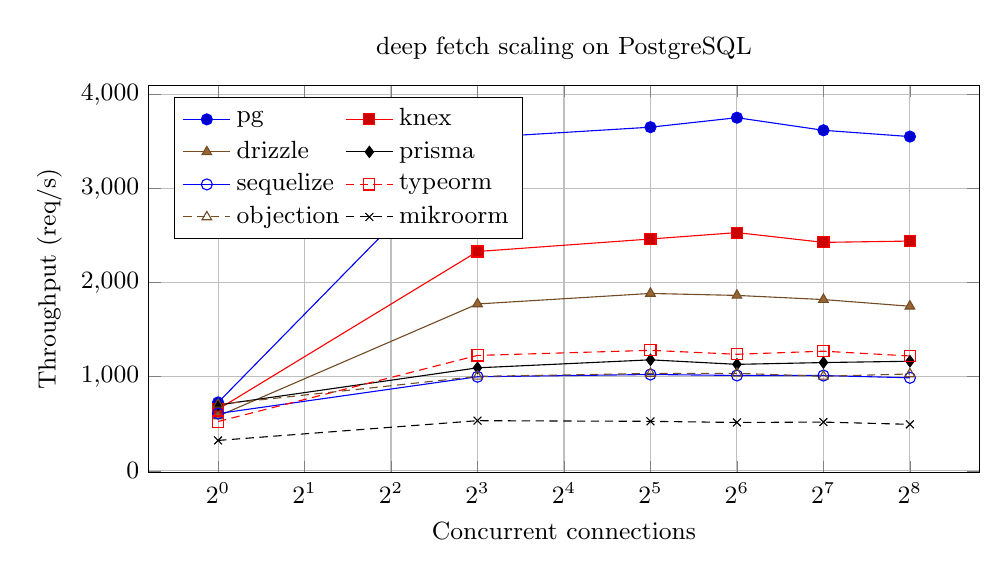
\begin{tikzpicture}
  \begin{axis}[width=\linewidth,height=6.5cm,xlabel={Concurrent connections},
      ylabel={Throughput (req/s)},xmode=log,log basis x=2,legend pos=north west,
      legend columns=2,legend cell align=left,font=\small,grid=both,
      title={deep fetch scaling on PostgreSQL}]
    \addplot+[mark=*] coordinates {(1,727) (8,3542) (32,3654) (64,3755) (128,3621) (256,3554)};
    \addlegendentry{pg}
    \addplot+[mark=square*] coordinates {(1,654) (8,2332) (32,2465) (64,2533) (128,2429) (256,2443)};
    \addlegendentry{knex}
    \addplot+[mark=triangle*] coordinates {(1,581) (8,1774) (32,1886) (64,1865) (128,1821) (256,1750)};
    \addlegendentry{drizzle}
    \addplot+[mark=diamond*] coordinates {(1,700) (8,1095) (32,1180) (64,1132) (128,1151) (256,1165)};
    \addlegendentry{prisma}
    \addplot+[mark=o] coordinates {(1,609) (8,1000) (32,1024) (64,1014) (128,1013) (256,989)};
    \addlegendentry{sequelize}
    \addplot+[mark=square] coordinates {(1,524) (8,1227) (32,1281) (64,1239) (128,1272) (256,1221)};
    \addlegendentry{typeorm}
    \addplot+[mark=triangle] coordinates {(1,706) (8,1004) (32,1035) (64,1036) (128,1005) (256,1030)};
    \addlegendentry{objection}
    \addplot+[mark=x] coordinates {(1,323) (8,533) (32,526) (64,514) (128,518) (256,494)};
    \addlegendentry{mikroorm}
  \end{axis}
  \end{tikzpicture}
  \caption{Deep-fetch throughput of each configured layer across the declared concurrency ladder (postgres). The curve maximum is used as an alternative empirical capacity denominator; uncertainty is assessed from the repeated point measurements.}
  \label{fig:scaling}
\end{figure}
